\chapter{Implementation}
\label{ch:implementation}

\section{Technology}
\label{se:tech}
While the design of the system specifies many architectural choices and sets out certain requirements for the implementation of the system, it leaves many options when it comes to the specific technologies used to create RT-Trainer. This section introduces and justifies the most important technologies used in RT-Trainer.

\subsection{Hosting}
\label{sse:hosting}
Firstly, the choice to host the system rather than just simply provide its code to potential users allows users to simply access a webserver hosting the system similarly to any other website they access on the internet. The obvious benefit of this is the benefit of web apps themselves - ease of access, hence hosting was used for this project. This does require the system to run on physical hardware, hence use computational resources. Luckily many web-hosting platforms offer free or "hobby" plans where usage is restricted but the features most "hobby" projects would require. These "hobby" plans act as a sort of free trial of features while the website doesn't exceed its resource limits, at which point the system is rate limited, stopped entirely or automatically upgraded to a paid plan. The latter type is uncommon and services which operate under this policy have not been considered. Similar plans exist for managed database platforms, logging platforms, and many other commonly used systems for developers, and hence have been used where appropriate such as a managed database (see section \ref{sse:database}). Justification of the use of other free plans is not made henceforth.

Various hosting providers offer minimal-configuration SvelteKit hosting, but the leading provider offering the most features is Vercel, which was chosen as the host of RT-Trainer. Many of the core contributors and the creator of Svelte were hired by Vercel to continue their work on Svelte, hence there is a clear commitment to supporting the framework into the future. Vercel offers a hobby plan for hosting, and numerous additional services with monthly limits at no charge such as a managed Postgres instance, various analytical tools and continuous deployment \cite{vercel-hobby-plan}. The limits imposed on the usage of the service were deemed as unlikely to be exceeded, but in that event, migration to another hosting provider with a free tier would have been a simple process.

\subsection{Database}
\label{sse:database}
As mentioned in the implementation section \ref{ch:implementation}, PostgreSQL was the chosen style of SQL database for storing user data (routes, scenarios). While many managed database providers offer PostgreSQL services, the provider with the most well documented and generous hobby plan was Planetscale. Although its DBMS supports only MySQL, not PostgreSQL, the original requirement for full geospatial data support was found to be unnecessary by this point in the project. The only geospatial data stored in the database was user generated waypoints, with all other aeronautical data fetched on demand from the OpenAIP API (see section \ref{se:aerodata}). Waypoint coordinates were stored as latitude and longitude in separate numeric type columns. Its limits of 10GB storage per month, 100 million row reads per month and 10 million row writes per month were deemed as unlikely to be exceeded.

Following an email from Planetscale indicating that they would retire the hobby plan on the 8th of April, weeks away from the project's final deadline, all data was migrated. Due to the limited time remaining in the project, the choice was made to move the data to Vercel's managed Postgres system as this would be quick to integrate into the project already hosted on Vercel. Due to the use of DrizzleORM (see section \ref{ssse:drizzle}) this migration was very quick.

\subsection{Supporting Libraries}
\label{sse:libraries}
As a means of accelerating development by reducing the amount of new code required to develop RT-Trainer, a number of libraries were used to support the new code written as part of this project. In general, they are all well documented, open-source, and actively maintained. Notable libraries are listed in this section, along with a description of their uses within RT-Trainer.

\subsubsection{Vite}
\label{ssse:vite}
It would have been possible to run SvelteKit's build step every time a minor change was made to the codebase, however with Vite, this was not required. Vite is a frontend build tool which supports Hot Module Replacement (HMR), allowing changes to be almost instantly present in the development server without running a slow, from scratch build command.

\subsubsection{Tailwind CSS}
\label{ssse:tailwind}
Tailwind is a CSS framework which simplifies the process of writing bespoke CSS, instead opting for a well design set of classes which can be added to the class of an HTML tag. For example \texttt{font-medium} works as shorthand for \texttt{\{font-weight: 500;\}}. The use of Tailwind meant minimal external CSS had to be written, instead placing the styling in the same place as the structure, where it could be though about at the same time, as the two concerns are managed easier together. Separation of concerns is a well know concept in the field of software engineering, but when it comes to the frontend, Tailwind finds a good balance of abstraction to not require it's separation from the UI structure.

\subsubsection{Skeleton UI}
\label{ssse:skeleton}
Skeleton provided both a basic shell app to build off of in a standardised way, but also a extensible library of UI components designed with usability in mind. Whenever a specific UI component was needed, Skeleton provided either the entire component pre-made, or the means to create it using a combination of its existing components. The use of a UI library meant that minimal time was spent working on aesthetic interfaces which users would appreciate, but are not the reason they are using the system. This is important, as poor UI design can turn potential users away \cite{}. Skeleton is built using Tailwind, and adds many more classes to Tailwind's base collection which meant that complex and aesthetic styling of components took just a couple of classes to create.

\subsubsection{Leaflet.js}
\label{ssse:leafletjs}
Performant and interactive maps are complex. Add the constraint of rendering in the browser and now you have very few libraries available. Leaflet is the leading open source option, with more than 11 years of updates, the minimal problems encountered were solved by finding a relevant blog post. The Leaflet library was very important to this project, with its map being used in more than half of the pages on the web-server.

\subsubsection{Turf.js}
\label{ssse:turfjs}
Turf simplified and standardised the geospatial computing required for features such as detecting airspace intersections and generating points some distance along a line. Originally all such methods were written from scratch using formulas found online, but minor mistakes lead to major bugs, so Turf was used to avoid these problems and improve the performance of route generation.

\subsubsection{DrizzleORM}
\label{ssse:drizzle}
While writing SQL queries is fairly simple for an application such as RT-Trainer, it would have taken a non-trivial amount of the project's duration to write, test and troubleshoot the required SQL queries. Object Relational Mapping tools exist to reduce the time developers spend dealing with the SQL model of their application's data, and allow them to interact with the data in a model much closer to that of their chosen language and framework. To this effect, DrizzleORM was used to abstract the database for the project and allow a greater focus on the novel features of RT-Trainer. Drizzle was chosen specifically for its edge-function support and DrizzleKit client which allowed easy management of rows and tables during development.

\subsubsection{Auth.js}
\label{ssse:authjs}
Logins, authentication and user data is a very important aspect of any system to get right. Auth.js is the industry standard open-source authentication library for Next.js, SvelteKit and Express, with many more frameworks supported. With OAuth support built in, RT-Trainer didn't need to store any usernames and passwords, instead login via OAuth providers was sufficient. Providing OAuth, where a user logs in via another account e.g. Google, Facebook, Microsoft is common in modern websites. It removes the risk related to sending passwords over the internet, or even storing them in RAM, and hence relies on the generally stronger security policies of the OAuth providers. Auth.js provides a suggested code snippet for use with DrizzleORM, endorsed by the maintainers of both libraries, which has been used in RT-Trainer to further reduce the risk of security vulnerabilities.

\subsubsection{Other Notable Libraries}
\label{se:otherlibraries}
In addition to the previously mentioned libraries, various other libraries used are listed below with a description of their use within RT-Trainer:
\begin{itemize}
    \item GeoJSON.js - Provided the language support for the types used by Turf.js \cite{GeoJSONNPM}.
    \item Axios - Provided a simple interface and boilerplate for API fetching \cite{AxiosNPM}.
    \item Leaflet.RotatedMarker - An extension for Leaflet.js allowing the rotating of markers, used to rotate the current location icon to the correct angle for the current point in flight \cite{LeafletRotatedMarkerNPM}.
    \item Svelte Icons Pack - A Svelte component based implementation of Flowbite's open source icon pack \cite{FlowbiteIcons}\cite{FlowbiteSvelteIconsNPM}. Used to improve usability by providing familiar controls to users.
    \item Vercel Web Analytics - Vercel's cookie-free analytical tool for monitoring site access metrics \cite{VercelWebAnalyiticsNPM}.
    \item Dotenv - Support for \texttt{.env} files for easy API and other secret key management. Various APIs used by the system require API keys or other secrets; Dotenv interfaces with Vite to ensure they are accessible, and only to the server \cite{DotenvNPM}.
\end{itemize}

\section{Aeronautical Data}
\label{se:aerodata}

% In order to have realistic data, need to get it from a decent source
Providing useful flight practice required using real world aeronautical data. Fortunately NATS distributes various Aeronautical Information Products (AIPs) on behalf of the UK Civil Aviation Authority \cite{NATS-Datasets}, which are for use in official charts and real world flight software. These files are published in a selection of CSV, XLS and XML formats once per month. Free APIs exist which provide endpoints for this data in a JSON format, which is more appropriate for RT-Trainer. OpenAIP is a community contribution based, Attribution-NonCommercial licensed AIP database with various tools and endpoints for accessing up-to-date flight planning data.

When a user accesses a page which requires data from OpenAIP, SvelteKit fetches the data from OpenAIP using Axios and passes it to the client in the \texttt{pageData} object, an optional object which can be included with any page in SvelteKit. This means that SvelteKit waits for the fetch to complete before sending the client the page. Filters are used to speed up the fetch, for example filtering to airspaces relevant for low altitude VFR flight, and all queries are filtered to only UK airspace, as OpenAIP is not limited to just the UK. While there is a wide selection of filters, there is no way to filter by a set of names, IDs or any other identifier. This causes certain fetches to take significantly longer than needed. When accessing a route that a user has created, the airports and airspaces along the route are known, and thus RT-Trainer only needs the data for these route features from OpenAIP. Despite this, it instead has to fetch all potential airports and airspaces and filter them after by ID. On a fast internet connection this is noticeable, and on slower connections causes some pages to take multiple seconds to load. Potential fixes are discussed in the conclusion chapter \ref{ch:conclusions}, but this issue has been left unresolved as meeting remaining system requirements has been the main priority.

The fetch process for the airspaces of a route takes the following steps:

\begin{itemize}
    \item Fetch required airspace IDs from the route's database row
    \item Construct a get request to https://api.core.openaip.net/api/airspaces using Axios with the OpenAIP access token injected from the \texttt{.env} file into the header, and filtered with parameters as follows:
    \begin{itemize}
        \item \texttt{country = `GB'}
        \item \texttt{iacoClass = [1, 2, 3, 4, 5, 6, 8]} (classes relevant for VFR)
        \item \texttt{onDemand = false}
        \item \texttt{onRequest = false}
        \item \texttt{byNotam = false}
    \end{itemize}
    \item Submit the request
    \item Receive the response
    \item If response is valid, cast the response data to AirspaceData objects (simple class with all of the same properties as the JSON data from OpenAIP so that types can be used)
    \item Filter the list of AirspaceData objects to contain only required airspaces
    \item Construct the remaining AirspaceData objects to Airspace objects, which have functions as well as data
\end{itemize}

% Include postman screenshot of a test - blur out api keys!

\section{Map Component}
\label{se:map}

Students taking the RT oral exam would be provided with a complete and detailed flight plan for their mock flight, hence the map component was designed in such a way to support sub-components which can be easily added. The leaflet library is fairly old when it comes to JavaScript libraries, and hence doesn't provide a component based API for use in modern frameworks, hence creating a component based Leaflet map was required. A tutorial by software consultancy firm Shipbit gave a good starting point for this, and was built on to support more features. This structural change came late in the project, after time was lost previously due to minor changes to the map code breaking other map features, but the change in structure roughly halved the code needed by the map while retaining all features. Other issues were encountered with the Leaflet library, including its use of coordinates in \texttt{(latitude, longitude)} form, rather than the GeoJSON standard \texttt{(longitude, latitude)} used by most modern geospatial libraries, including Turf.js \cite{GeoJSONRFC}.

The map effectively works by internally connecting the Leaflet library code to a Svelte component, which has a slot tag. Slot tags allow other components to be nested within the original component, for example a marker component within a map component. This map component would interface with the leaflet library, but be bound to the its svelte component, such that creating a marker Svelte component with some properties would create a marker on the Leaflet map with those properties. This is how most libraries which are not component based UI libraries already, are turned into components in Svelte, and other component based frameworks. By keeping all frontend libraries component based in a codebase, complexity is reduced as the only way to display something is via a component, thus interactions are generally simple to understand.

\begin{figure}
    \centering
    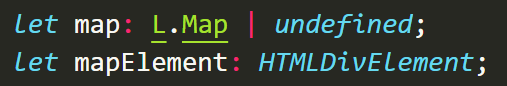
\includegraphics[width=0.25\linewidth]{document-resources//images/map-leaflet-variables.png}
    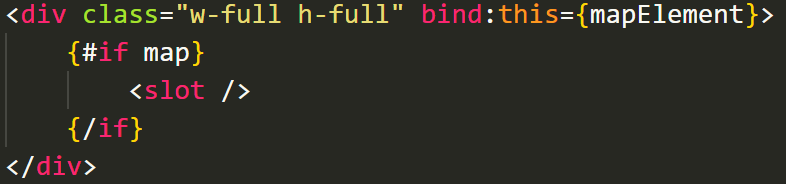
\includegraphics[width=0.25\linewidth]{document-resources//images/map-svelte-component-rough.png}
    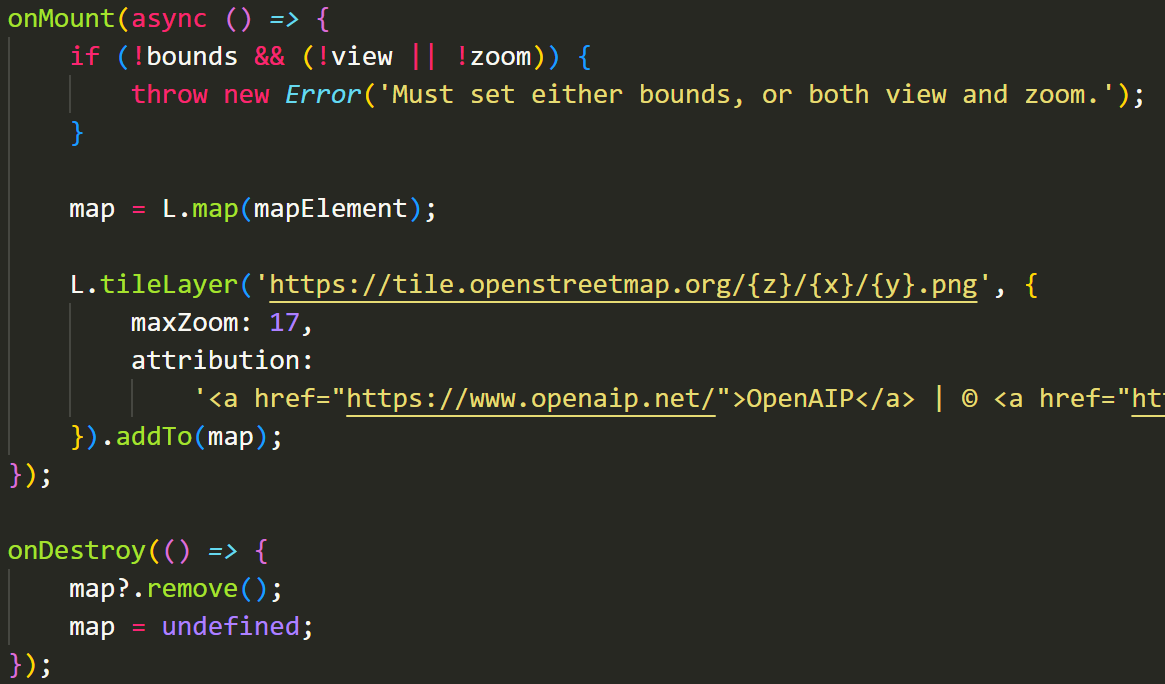
\includegraphics[width=0.25\linewidth]{document-resources//images/map-onmount.png}
    \caption{Svelte code for map component showing slot tag and binding property tied to underlying Leaflet map. \texttt{onMount} connects the Leaflet map to the component, and \texttt{onDestroy} removes it when the component is destroyed in order to correctly handle resources, reducing the chance of a memory leak.}
    \label{fig:map-svelte-component}
\end{figure}

To support the drawing of a flight path, airspaces, airports, headings, and other requirements of the flight plan, marker, polyline (straight lines connecting a sequence of points), polygon, popup and control components were developed in a similar way to the component based map. Each component has a slot tag, just like the map. For the polyline, polygon and marker these are used to add popups, and for the popup and control components, the slot is used to add further Svelte components such as HTML to show current heading. 

\section{Routes}
\label{se:routes}
As mentioned in the design section, a route is a sequence of waypoints and is created by a user, with the ability to then be used in a scenario. Internally, a route in RT-Trainer is simply defined as a \texttt{RouteData} object, comprising a list of waypoints, airports and airspaces.

\subsection{Route Generation}
\label{sse:routegen}

Route generation requires fetching data required to construct a route, and computing a route close enough to an exam route to be useful to users. Initially this was all performed by a separate webserver, written in Rust, with the result sent to the frontend. Although this was very performant, the exact process of route generation had not been finalised, and was expected to undergo many changes as more was learned about both the constraints of exam routes, and the design of the frontend. Due to this, when returning to the project after taking a break to complete other coursework over the winter break, all rust code was ported to TypeScript and made part of what was initially the frontend webserver. TypeScript proved much better for quickly iterating versions, given that it doesn't have a slow compilation time, has access to many more libraries and can be run with syntactic errors. 

% Actual technical shit about the route gen

\subsection{Route Planner}
\label{sse:routeplanner}

The first hosted version of RT-Trainer featured only the route generator, and no manual route planner, as this was the original design. However, late into the project, it became clear that the usefulness of the system would be greatly improved by its inclusion, and that most of the groundwork had already been completed to support it. 

The route planner is in the form of a page mostly taken up by a map component, featuring all relevant UK airports and airspaces, and an information sidebar and footer. The sidebar features a summary of the route waypoints, with the ability to change names, delete or drag to re-order. The sidebar also features controls to change distance unit, maximum flight level and a way to invoke the route generator based on a seed the user can input. Finally, the footer shows the estimated route distance and number of airspaces included on-route.

A user creates a route by clicking anywhere on the map to define a waypoint. If an airport is clicked, it is marked as a waypoint, meaning that the scenario generator can later down the line use the data on the airport to properly generate scenario points for takeoff or landing. Clicking anywhere else will create an airborne waypoint, modelled as being at the maximum flight level for the route, e.g. 3000ft or FL30. Waypoints are connected in order by straight lines, which is standard for flight planning software \cite{SkyDemon}\cite{SkyVector}, and feature an icon which can be dragged to a new location (as long as the waypoint is not at an airport). Clicking on a waypoint shows a popup giving the user the ability to change its name, latitude and longitude, or to delete it entirely. Edit controls are not shown for airport waypoints.

When the ``Save Route" button is clicked, a modal appears requiring the user to input a name and set the route visibility, and gives the option to add a route description. The visibility option determines whether other users should be able to view the route, and how they will find it. \texttt{Public} allows the route to show up in the public routes list, \texttt{Unlisted} routes are only accessible by accessing its URL, and \texttt{Private} routes can only be seen by the creator themselves (the default option). Once submitted the route is saved to the database via an API call to the \texttt{/route} endpoint. As long as this API post request is successfully validated, a route with its details is pushed to the database, followed by its waypoints with foreign keys linking back to the route. References to the airports and airspaces along the route are also stored, meaning the system need not load all and determine which it actually needs to display every time the route must be shown, instead it can simply fetch only those which are needed.

\section{Scenario Generation}
\label{se:scenariogen}

\subsection{Scenario Points}
\label{sse:scenariopoints}

\subsection{Weather Model}
\label{sse:metormodel}
An important detail included in many radio calls is the current pressure. As well as this, certain radio calls also contain other weather details, hence a suitable realistic weather model was developed in order to provide this data for radio call generation. A seeded normal distribution was used to generate the required values whenever required, and the mean and standard deviation of the random variables is determined entirely by the seed.

Each airport has a METOR data sample associated, which is created when the airport object is instantiated. The mean and standard deviation values for each variable are determined by the latitude, longitude and elevation of the airport.
% The calculation should be improved before writing this lol, its super crude and writing much about it will be a mess. It needs validating via testing. Could ask chatgpt for a better one

First the seed is used to determine the season. This ensures that there can be variance between points along the route where meteorological data is required, while keeping the values close enough to be believable. 

\section{Simulator}
\label{se:sim}

\subsection{Input and Output Radio Calls}
\label{sse:inputoutput}

\subsection{Radio and Transponder}
\label{sse:radiotransponder}
% Remember that the design will have been discussed already in the design section
The radio and transponder are Svelte components with various sub-components, properties and functions to allow them to mimic their real life counterparts. For example, various dial components were created, which allow a user to click on a side of the dial for it to turn either clockwise or anticlockwise, with these turn events being subscribed to by the parent component, in order to adjust a value displayed. By these means a user can change the frequencies of the radio and transponder in a way similar to real life. By using the JavaScript \texttt{setInterval} function, clicking and holding down on one side of a dial will continuously turn it, triggering the relevant rotate event more and more frequently the longer it is held. Combining this with non-held clicks, both speed and accuracy can be achieved when adjusting frequencies, while keeping the interactions similar to real life dials.

\begin{figure}
    \centering
    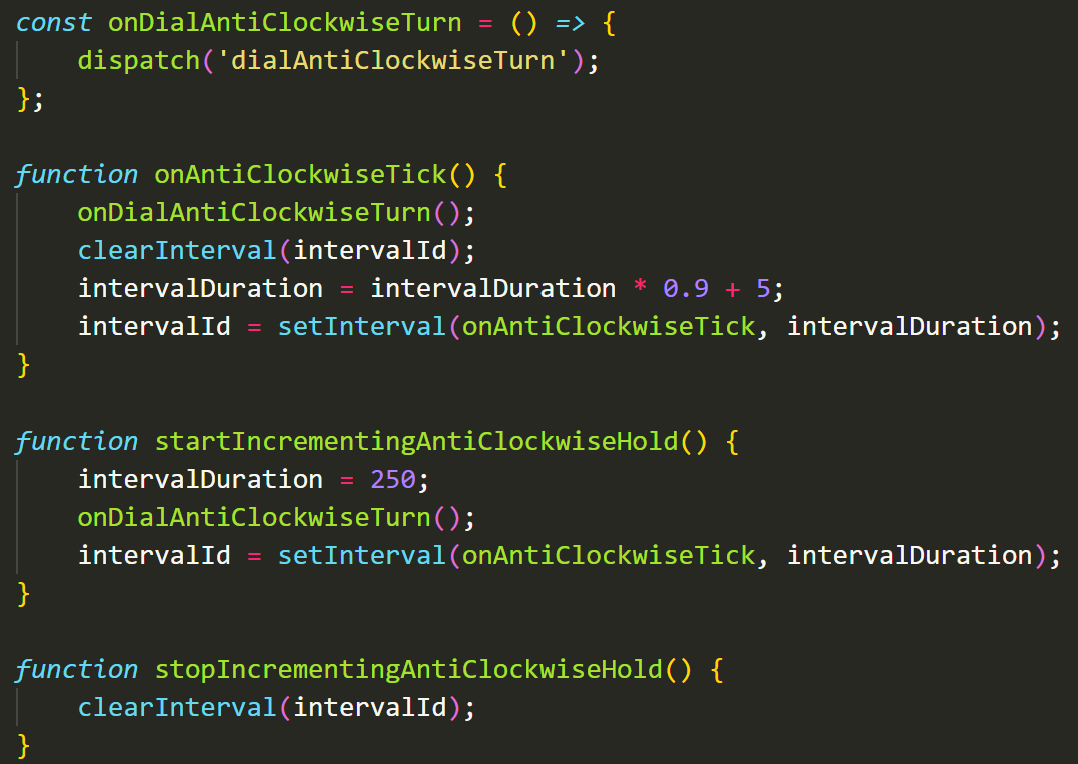
\includegraphics[width=0.5\linewidth]{document-resources//images/dial-turn-code.png}
    \caption{Enter Caption}
    \label{fig:enter-label}
\end{figure}

Seven segment display components were developed to act as displays for the frequency of both the radio and transponder, which stylistically are effectively a glowing seven segment font. Displaying the correct values however required a lot more work. Due to the way computers store numbers, the numerical frequency cannot not be displayed directly, given that the number $118.300$ would be displayed as $118.3$. Partially for redundancy in often poorly readable radio calls, the full frequency, including proceeding or trailing zeros should be stated. Real life radios and transponders reflect this by always displaying the same number of digits. Therefore a string version of the frequency is displayed for the radio display, and a digit array, displayed digit by digit, is used for the transponder display, as its workings are slightly different. The transponder's dial adjust the frequency of only the selected digit, with buttons to move the digit selector. This design means that numeric values can be directly displayed.

\subsection{Altimeter}
\label{sse:altimeter}

The altimeter was a suggestion by the project's client, who proposed that it replace the kneeboard which was simply a note taking text box in the same position on the page. An important part of VFR flight is the calibration of the altimeter, which is based on the current pressure reading. The further from the correct pressure the altimeter is set, the more inaccurate its readings become. Therefore the integration of the altimeter allows users to practice setting the current pressure reading when it is given to them in a radio call, in order to get the correct current altitude.

The HTML, CSS and SVG images which make up the visuals of the altimeter were published by Peter Shmulevich under the MIT license \cite{altimeter-codepen}.

\section{Radio Call Parsing}
\label{se:parsing}
% Feedback

\section{Authentication and Authorisation}
\label{se:authauthor}
% Which pages are protected, why and how
